\documentclass[12pt,a4paper]{article}
\usepackage[left=3cm,right=2.5cm,top=3cm,bottom=3cm]{geometry}
\usepackage{tabularx}
\usepackage{titlesec}
\usepackage{sectsty}
\usepackage{graphicx}
\usepackage{float}

\floatstyle{plain}

\sectionfont{\fontsize{12}{15}\selectfont}
\subsectionfont{\fontsize{12}{15}\selectfont}
\titlelabel{\thesection. }

\newcommand*{\details}[3]{
  \textbf{#1}&\textbf{#2}&: #3 \\
}
\newcommand*{\br}[3]{
  \textbf{#1}&\textbf{#2}& #3 \\
}
\newcommand{\specialcell}[2][t]{%
  \begin{tabular}[#1]{@{}l@{}}#2\end{tabular}}
\begin{document}
\thispagestyle{empty}
\begin{center}
\large \textbf{Chittagong Universioty of Engineering \& Technology}\break
\large \textbf{Department of Computer Science \& Engineering}\break
\large \textbf{Chittagong-4349}\break
\break
\normalsize \textbf{(Project/Thesis Proposal)}\break
\break
\textbf{Application for the approval of B. Sc. Engineering Project/Thesis}\\
\textbf{(Computer Science \& Engineering)}
\end{center}
\begin{flushright} \textbf{Date: 23-9-2019} \end{flushright}
\begin{tabular}{ll@{\hspace{1cm}}l}
\br{}{}{}
\details{1.}{Name of the Student}{Simon Islam}
\details{}{Roll No.}{1504062}
\details{}{Session}{2018-2019}
\br{}{}{}
\details{2.}{Present Address}{\specialcell{Room No: 110\\Shahid Tarek Huda Hall\\Chittagong University of Engineering \& Technology\\Chittagong-4349}}
\br{}{}{}
\details{3.}{Name of the Supervisor}{Animesh Chandra Roy}
\details{}{Designation}{\specialcell{Assistant Professor\\Department of Computer Science \& Engineering\\Chittagong University of Engineering \& Technology\\Chittagong-4349}}
\br{}{}{}
\details{4.}{Name of the Department}{Computer Science \& Engineering}
\details{}{Program}{B.Sc. Engineering}
\br{}{}{}
\details{5.}{\specialcell{Date of First Enrollment\\in the Program}}{25 February, 2016}
\br{}{}{}
\details{6.}{Tentative Title}{\specialcell{Multi-Label Emotion Classification on Trending Tweets \\using Machine Learning}}
\end{tabular}
\pagebreak
\setcounter{section}{6}
\section{Introduction}
\par \noindent Twitter is currently one of the biggest social network in the world. As of september, 2019, it has 330 million active users worldwide. It is famous for it's microblogging feature. Microblogging is the habit of making tiny posts to a microblog. It can range from various topics, pictures, gifs or sharing a link. Before november, 2017, a user can write a tweet consists of at most 140 characters. But since then, twitter has doubled this capacity to 280 characters. When comparing with other social media giants like facebook, the characteristics that sets twitter apart is it's reach. Twitter has a global reach. It is not limited to friends and family. Instead, it encompasses the poster and his follwers. In other social network sites like facebook, if someone wants to see someone's posts both has to accept each other as friends. But in twitter all someone has to do is to follow the other person. This one way follower relationship has given twitter a global reach. 
\par \noindent In today's world, trends are changing on daily basis. Twitter detects this current trends by calculating the volume of a keyword over a period of time. The spike in the volume in a short time classify the keyword as trends. And the tweets having those keywords in that time are called trending tweet. Due to twitter having this global reach \& vast number of users, it has become a global platform to express peoples emotion online. From average day people to superstars, everyone use twitter to express their emotions on various topics. In return, their followers gives a feedback of his own emotions. To understands what kind of sentiments are they creating around the world, it is important to be able to extract emotions from their tweets. It can help researchers to understand how people are feeling about a certain topic.  During the recent age of social media, sentiment analysis has been one the most studied field by the researchers. It is the process of identifying and categorizing sentiments over a piece of text. It extracts valuable features from the texts. Sometimes confused with opinion mining, sentiment analysis deals with sentiments of the text where in opinion mining extract opinion.
\par \noindent In this work, we aim to perform multi-label emotion analysis of tweets posted in twitter. We wish to classify the tweets in one of 8 emotion classes. They are: sadness, disgust, joy, interest, admiration, anger, surprise \& fear. We will collect trending tweets from twitter and will try to label them with emotions that describe them best. It is a multi-label classification because more than one emotion may be needed to properly clssify a tweet. Although many work has been done on sentiment analysis, very few of them attempted to classify them in multiple labels. Our main goal in this work is to properly label them accoring to their emotional sentiments.

\section{Background and Present State of the Problem}
\par \noindent In this current age of social media, people has began to discuss their thoughts, daily lives and works on social media. They comment on various happenings around the world and how it is affecting their lives or the lives of other people. This huge dependency of peole on social media has attracted researchers to study the behaviors. Twitter, due to it's global reach and accessibility has attracted many researchers. Some of the researches include the use of slangs, emoticons and how they developed over a period of time.\cite{1,2} Most of the sentiment analysis done on twitter has been binary classification. In binary classification, the tweets are marked from negative to positive. Some classification also contains a neutral class. They include polarity of products\cite{3}, movies\cite{4} and democratic election.\cite{5} There are also some advanced work that went deeper into the classification and tried to asses the strength of the sentiment. Their range included from very negative to very positive, in some cases giving scores depending on the sentiment intensity.\cite{6,7} 
\par \noindent In the recent years, the works on multi-label classification has started to gain some traction. Instead of labelling a tweet positive, negative or neutral, a multi-class classification labels it according to the emotions found in the text. Bhowmick, Basu et al.\cite{8} used multilabel sentiment classification on news extracted from Times of India newspaper. Liu et al.\cite{9} used a multi-label classification approach to perform multi-label classification of microblogs. They performed this on gatherd data. Bouazizi et al.\cite{10} used 3 pairs of opposite sentiment to label their tweets. They didn't consider statements of opposite polarity. We wish to perform multi-label emotion classification on real time trending tweets on twitter.

\section{Aims with Specific Objectives \& Possible Outcomes}
\par \noindent The main objectives \& the possible outcomes of this work are mentioned in the following:
\begin{itemize}
\item To extract real time trending tweets from twitter
\item To perform Multi-Label Emotion Analysis of the tweets (sadness, disgust, joy, interest, admiration, anger, surprise \& fear)
\end{itemize}
\section{Outline of Methodology}
\par \noindent  The key objective of our work is to develop a system that can process the tweets and label them according to their emotions. We first need to gather a dataset of tweets. Twitter provides their own api that can collect tweets from twitter. Then we need to clean the dataset. We do this by removing links and pictures from the tweets. Then we separate the senteces, hashtags, emoticons from the tweets. From the senteces, we will detect phrases, expand emoticons, process elongations. We also need to detect negation in a sentence or does it represent two different emotions with conjunctions.  For this, we need to consider each and every tweet individually and preprocess it before sending it to train our model. Another important step before the training is feature extraction. When all the steps are finally complete, we use our data to train multi-label sentiment classification model. Finally, the model is tested using the test cases that we create.And it will be evaluated and deployed in a real time enviroment, where it will detect emotions in currently trending tweets. A brief overview of our system is given below:
\begin{figure}[H]
	\centering
	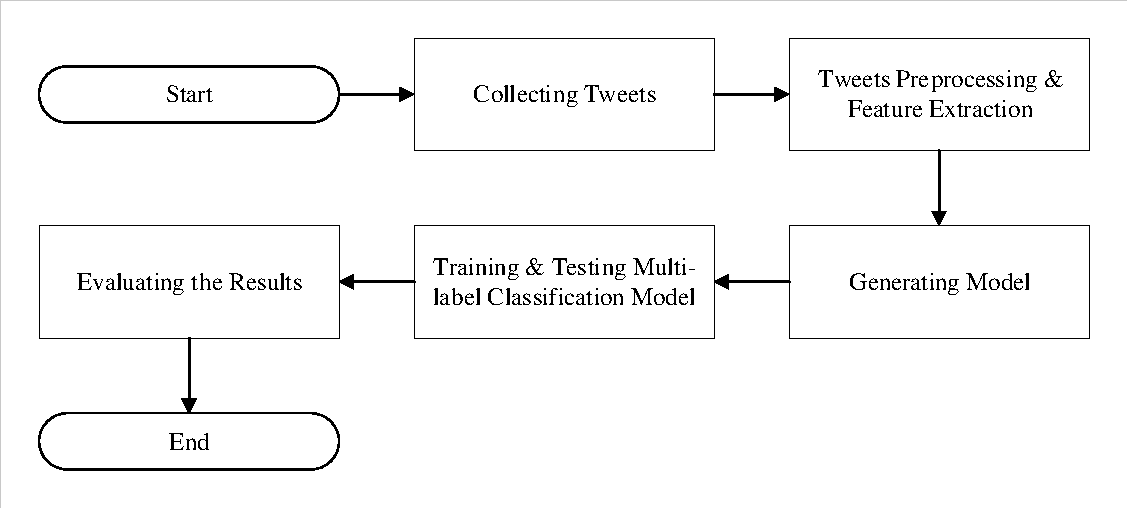
\includegraphics[scale=0.8]{1-1.pdf} \qquad
	\caption{Overview of the work}
	\label{1}
\end{figure}
\subsection*{Collecting Tweets}
Twitter has it's own API that can be used to collect tweets from twitter. It can be used to collect data in real time or from a selected user or regarding a specific topic. We will use it to collect tweets in real time.
\subsection*{Preprocessing Tweets}
To be able to train our model, it is important to process our data properly. Unlike a sentence, a tweet is not a collection of words. People uses sentences, punctuations, phrases, acronyms, emoticons to properly convey their messages. Our job here is to process the text in a way to make it clean. And we will also extract features from other aspects of tweet. Data preprocessing phase is described as follows:
\begin{itemize}
\item Remove pictures, web links and e-mails
\item Separate sentences, punctuations, hashtags \& emoticons
\item Process the hashtag to seperate it by words
\item Count the number of question marks and exclamation mark after each word
\item Expand the acronyms \& parts of speech tagging
\item Recognize intensifier word classes and negation words
\item Remove stopwords, process elongation \& perform word stemming and lemmatisation of word
\item Map the emoticons according to their emotions
\end{itemize}
\begin{figure}[H]
	\centering
	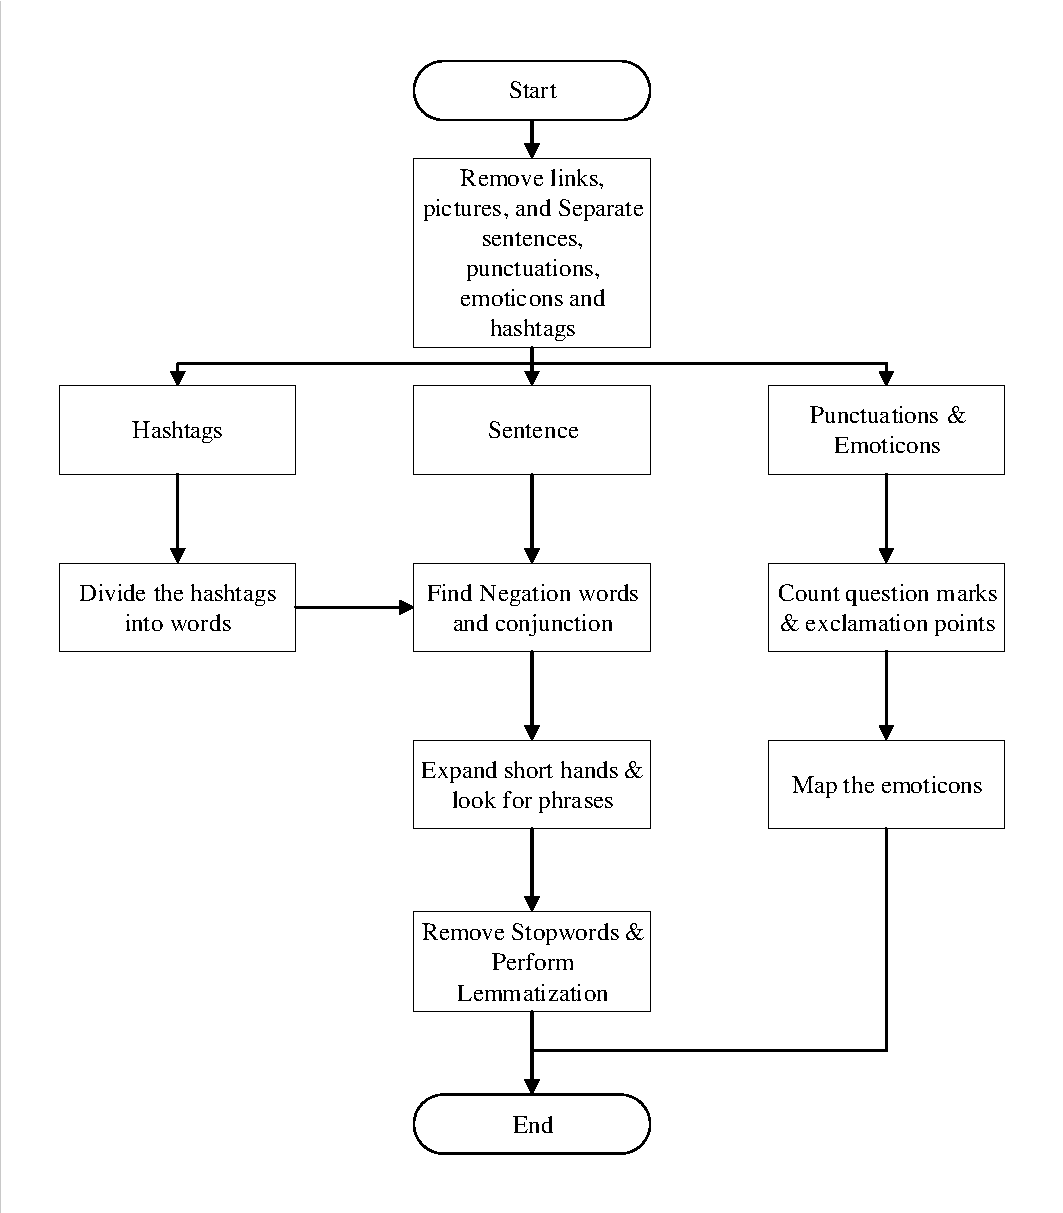
\includegraphics[scale=0.7]{2-1.pdf} \qquad
	\caption{Tweet Preprocessing Flowchart}
	\label{2}
\end{figure}
\subsection*{Training and Testing the Data}
There are two ways to approach sentiment analysis. One is lexicon based and the other is machine learning based. In the our work, we wish to perform multi-label emotion classification using machine learning. There are many machine learning algorithms that are suited for this work. Some of them being Naive Bayes, SVM, Maximum Entropy, Long-short term memory etc. In this step we label the data and train our model. For the labelling purpose we would like to use established datasets. But if such datasets are not found then we will propose our own labelling method to perform multi-level sentiment analysis. For that case, we will use various sentiment libraries like SenticNet \cite{11} and others. Then finally we test the model against our testing data. 
\begin{figure}[H]
	\centering
	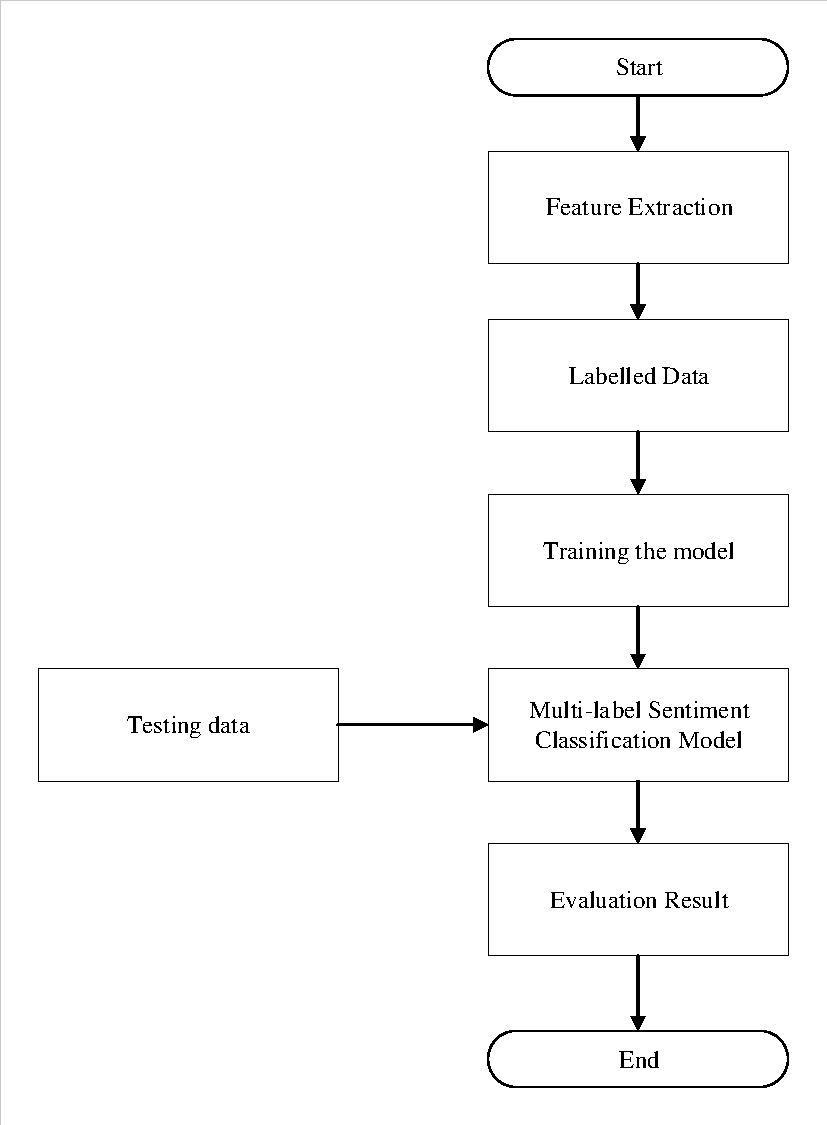
\includegraphics[scale=0.8]{3-1.pdf} \qquad
	\caption{Multi-label Sentiment Classification Model}
	\label{3}
\end{figure}

\section{Resources Required to Complete the Work}
\par \noindent The resources required to complete the work can be divided into two categories. They are hardwares and software. The requirements are illustrated below:
\begin{itemize}
\item \textbf{Hardware Components} 
\begin{itemize}
\item Personal Computer
\end{itemize}
\item \textbf{Software Components}
\begin{itemize}
\item Python 3.7
\item PyCharm IDE for Python
\end{itemize}
\end{itemize}

\section{Cost Estimate}
\par \noindent The cost that will occor to complete our proposed work is given below:
\subsection*{Cost of Materials:}
\begin{tabular}{l@{\hspace{9cm}}lr}
\br{}{}{}
A general laptop &Tk.&50000\\
\br{}{}{}
Paper &Tk.&500\\
\br{}{}{}
\textbf{Total}&\textbf{Tk.}&\textbf{50500}
\end{tabular}
\subsection*{Typing, Drafting, Binding:}
\begin{tabular}{l@{\hspace{6.87cm}}lr}
\br{}{}{}
Internet Browsing \& Typing &Tk.&2500\\
\br{}{}{}
Drafting&Tk.&500\\
\br{}{}{}
Binding&Tk.&500\\
\br{}{}{}
\textbf{Total}&\textbf{Tk.}&\textbf{3500}\\
\br{}{}{}
\textbf{Grand Total}&\textbf{Tk.}&\textbf{54500}\\
\end{tabular}

\pagebreak

\bibliographystyle{ieeetran}
\bibliography{ref}
\pagebreak
\section{CSE Undergraduate Studies (CUGS) Committee Reference}
\begin{tabular}{l@{\hspace{3cm}}l@{\hspace{3cm}}l}
\textbf{Meeting No.:}&\textbf{Resolution No.:}&\textbf{Date:}\\
\end{tabular}
\section{Number of Undergraduate Students working with the Supervisor at Present: 2}
\begin{flushright}
\bigskip
\bigskip
\begin{minipage}{6cm}
\begin{tabular}{c}
\makebox[2.5in]{\hrulefill}\\
Signature of the Student\\[8ex]
\makebox[2.5in]{\hrulefill}\\
Signature of the Supervisor\\[8ex]
\makebox[2.5in]{\hrulefill}\\
Signature of the Head of the Department\\
\end{tabular}
\end{minipage}
\end{flushright}
\end{document}